\documentclass[a4paper]{article}
\usepackage[portuguese]{babel}
\usepackage[utf8x]{inputenc}
\usepackage[T1]{fontenc}
\usepackage[ddmmyyyy]{datetime}
\usepackage{array}
\usepackage{xcolor}
\usepackage{listings}
\usepackage{verbatim}
\usepackage[a4paper]{geometry}
\usepackage{amsmath}
\usepackage{natbib}
\usepackage{graphicx}
\usepackage{fancybox, graphicx}
\usepackage{float}
\usepackage[colorinlistoftodos]{todonotes}
\usepackage[colorlinks=true, linkcolor=blue, urlcolor=red]{hyperref}
\usepackage{fontspec}
\defaultfontfeatures{LetterSpace=1.5}
\setmainfont{Times New Roman}
\lstset{basicstyle=\ttfamily, showstringspaces=false, commentstyle=\color{red}, keywordstyle=\color{blue}}

\begin{document}

\begin{figure}[!t]
    \centering
    
\includegraphics[scale=0.55]{figuras/estig.png}
\end{figure}

\title{Interação Pessoa Computador\\1º Trabalho de Grupo\\\textit{EasyMed}}
\author{Ricardo Sequeira - 21905 \\ Sebastião Pereira - 21932 \\ Diogo Guerreiro - 17435}
\date{\today}

\maketitle

\pagebreak

\tableofcontents
\listoffigures

\pagebreak

\section{Introdução}
O presente relatório apresenta o \textit{design} e funcionalidades decididas para a \textit{EasyMed}, uma aplicação com o objectivo lembrar os utilizadores dos medicamentos que estão a tomar, com bastante ênfase na simplicidade e acessibilidade.\\
O relatório esta divido em 10 capítulos e os respectivos subcapítulos na caracterização dos utilizadores alvo (\ref{section:carac_users}), uma análise de sistemas semelhantes (\ref{section:similar_analysis}), os cenários de utilização previstos (\ref{section:use_cases}), as analises de tarefas referentes aos cenários anteriores (\ref{section:chores_analysis}), as funcionalidades que pretendemos implementar (\ref{section:features}), e para que tipo de dispositivos móveis as implementaremos (\ref{section:style_n_use}), os protótipos de ecrãs de baixa e alta fidelidade (\ref{section:app_prototype}) as regras de usabilidade aplicáveis (\ref{section:usability_rules}) na nossa proposta e a conclusão (\ref{section:summary}).

\section{Caracterização dos Utilizadores}\label{section:carac_users}

\subsection{Personas}
Nesta secção vamos apresentar alguns possíveis tipos de utilizadores para a nossa aplicação.

\begin{center}
Persona Um:
\end{center}

\begin{itemize}
    \item Idade: 24
    \item Identidade Sexual: Masculino
    \item Nível de Escolaridade: Ensino Secundário
    \item Profissão: Estudante
    \item Experiência Informática: Utilizador Experiente
    \item Quanto tempo passa em média no seu dispositivo móvel diariamente(horas): 5-6 horas
    \item Que funcionalidades gostaria de ver na aplicação \textit{EasyMed}: Guardar a imagem de cada comprimido para ser mais fácil e rápido reconhecer os medicamentos.
    \item Que funcionalidades de acessibilidade acha que devem ser implementadas nesta aplicação: Text-to-speech para ler o nome dos comprimidos

\end{itemize}

\begin{center}
Persona Dois:
\end{center}

\begin{itemize}
    \item Idade: 60
    \item Identidade Sexual: Feminino
    \item Nível de Escolaridade: Licenciatura
    \item Profissão: Técnica de Informática
    \item Experiência Informática: Entusiasta
    \item Quanto tempo passa em média no seu dispositivo móvel diariamente(horas): 7+ horas
    \item Que funcionalidades gostaria de ver na aplicação \textit{EasyMed}: Possibilidade de lembretes para comprimidos de múltiplas tomas diárias
    \item Que funcionalidades de acessibilidade acha que devem ser implementadas nesta aplicação: N/A
\end{itemize}

\begin{center}
Persona Três:
\end{center}

\begin{itemize}
    \item Idade: 30
    \item Identidade Sexual: Não Binárie
    \item Nível de Escolaridade: Ensino Básico
    \item Profissão: Barbeiro
    \item Experiência Informática: Utilizador Básico
    \item Quanto tempo passa em média no seu dispositivo móvel diariamente(horas): 3-4 horas
    \item Que funcionalidades gostaria de ver na aplicação \textit{EasyMed}: Notificações Pop-Up
    \item Que funcionalidades de acessibilidade acha que devem ser implementadas nesta aplicação:\\
    Haver bloqueio na aplicação para prevenir alterações descuidadas
\end{itemize}

\begin{center}
Persona Quatro:
\end{center}

\begin{itemize}
    \item Idade: 42 
    \item Identidade Sexual: Masculino
    \item Nível de Escolaridade: Ensino Secundário
    \item Profissão: Guarda Rios
    \item Experiência Informática: Utilizador Básico 
    \item Quanto tempo passa em média no seu dispositivo móvel diariamente(horas): 1-2 horas
    \item Que funcionalidades gostaria de ver na aplicação \textit{EasyMed}: N/A
    \item Que funcionalidades de acessibilidade acha que devem ser implementadas nesta aplicação: N/A
\end{itemize}

\subsection{Questionário}
Para podermos obter um maior conhecimento das necessidades dos nosso utilizadores decidimos também criar um questionário com as seguintes questões:
\cite{gforms_easymed}

\begin{enumerate}
    \item Idade;
    \item Identidade Sexual;
    \item Nível de Escolaridade;
    \item Profissão;
    \item Experiência Informática;
    \item Quanto tempo passa em média no seu dispositivo móvel diariamente(horas);
    \item Que funcionalidades gostaria de ver na aplicação \textit{EasyMed};
    \item Que funcionalidades de acessibilidade acha que devem ser implementadas nesta aplicação.
\end{enumerate}

\vspace{1cm}
Como a Experiencia Informática é a única questão que é subjectiva que utilizamos uma escala de um a cinco: 
\begin{enumerate}
    \item Tecnologicamente Iletrado
    \item Utilizador Básico
    \item Utilizador Experiente
    \item Entusiasta
    \item Utilizador e programador experiente
\end{enumerate}

\section{Sistemas Semelhantes}\label{section:similar_analysis}
As aplicações seguintes são algumas mais populares e semelhantes no género da nossa aplicação, iremos mostrar algumas das suas vantagens e desvantagens, para que possamos aplicar alguns desses conhecimentos no desenvolvimento da nossa própria aplicação. \cite{sim_apps}

\subsection{\textit{MediSafe} - Vantagens e Desvantagens}

\begin{itemize}
    \item Permite que o utilizador seja informado caso duas ou mais das medicações que tem para ser tomadas são incompatíveis, evitando assim efeitos secundários graves.
    \item Permite armazenar na \textit{cloud} as informações relevantes a medicamentos e lembretes, assim caso o utilizador mude de dispositivo todos as informações da sua conta estarão disponíveis.
    \item Tem como desvantagem não permitir que as notificações tenham som com o modo silencioso ligado, obrigando assim os utilizadores a terem sempre o telemóvel com o som ligado o que pode ser uma inconveniência para muitos utilizadores.
\end{itemize}

\subsection{\textit{MangoHealth} - Vantagens e Desvantagens}

\begin{itemize}
    \item Permite aos utilizadores customização total do seus horários de toma de medicações, permitindo por exemplo para um comprimido de toma diária definir uma hora de toma mais tardia aos fins de semana.
    \item Permite também aos utilizadores não só lembretes de medicações, mas também de outros hábitos de saúde como por exemplo notificações de hidratação e de medição de glucose no sangue no caso dos diabéticos.
    \item Tem como desvantagem apenas permitir introdução manual dos medicamentos e dos hábitos acima mencionados, ao invés de outras aplicações que permitem fazer \textit{scan} do código de barras dos medicamentos ou até conexão com a farmácia em si. 
\end{itemize}

\subsection{\textit{RoundHealth} - Vantagens e Desvantagens}

\begin{itemize}
    \item Permite aos utilizadores não só inserir todas as medicações receitadas como as as aplicações acima mencionadas, mas tem também a funcionalidade de notificar quando a medicação está quase a terminar para que o utilizador se possa dirigir à farmácia para comprar mais.
    \item Esta aplicação permites aos seu utilizadores que a usem sem a necessidade de criação de uma conta, o que é bom para quem está preocupado com a sua segurança \textit{online}.
    \item Tem como desvantagem que em medicações com várias tomas diárias, por exemplo de 8 em 8 horas, o utilizador tem que criar lembretes para cada uma das tomas.
\end{itemize}

\section{Cenários de Utilização}\label{section:use_cases}
Nesta secção iremos mostrar alguns cenários de utilização mais comuns para os utilizadores na nossa aplicação. \cite{usecases}

\begin{itemize}
    \item O utilizador quer adicionar um lembrete de um medicamento à aplicação \textit{EasyMed}.
    \item O utilizador quer alterar o horário da toma do medicamento na aplicação \textit{EasyMed}.
    \item O médico/cuidador quer fazer alterações à guia de medicações do seu paciente na aplicação \textit{EasyMed}.
\end{itemize}

\section{Análise de Tarefas}\label{section:chores_analysis}
Nesta secção iremos descrever como são efetuados os cenários de utilização descritos no ponto anterior.

\subsection{O utilizador quer adicionar um lembrete de um medicamento à aplicação \textit{EasyMed}}
No ecrã inicial da aplicação (\ref{fig:second_screen_main_screen}) iremos implementar um \textit{UI} com um botão de mais (+) que seguirá para um ecrã que permitirá inserir os detalhes do medicamento a ser adicionado.

\subsection{O utilizador quer alterar o horário da toma do medicamento na aplicação \textit{EasyMed}}
Para editar o horário ou qualquer outra informação referente ao lembrete, basta clicar no mesmo no ecrã inicial da aplicação (\ref{fig:second_screen_main_screen}) e será mostrado um ecrã semelhante ao de adição de lembretes (\ref{fig:third_screen_add_remainder}) com todas as informações referentes ao lembrete.

\subsection{O médico/enfermeiro quer fazer alterações à guia de medicações do seu paciente na aplicação EasyMed.}
Para evitar que pessoas que sejam mais "descuidadas" pretendemos aplicar um bloqueio nas definições e modificações dos medicamentos ou dos seus horários.
Para ativar este bloqueio basta aceder às definições que se vão encontrar no ecrã principal da aplicação. (\ref{fig:second_screen_main_screen})


\section{Funcionalidades da Aplicação}\label{section:features}
Nesta secção vamos descrever algumas funcionalidades que gostaríamos de implementar e ver implementadas numa fase seguinte de desenvolvimento.

\begin{itemize}
    \item A aplicação irá ter a funcionalidade que permitirá a um medico/cuidador 
    bloquear a aplicação com um código de 4 dígitos de modo a não permitir a utilizador com problemas de acessibilidade apagar lembretes importantes ou fazer alterações erradas;
    \item A aplicação irá permitir o utilizador receber notificações estilo alarme, com \textit{pop-up}, de modo a alertar o utilizador acerca da medicação a tomar caso o mesmo não se encontre dentro da aplicação nesse dado momento;
    \item A aplicação irá permitir guardar uma fotografia do medicamento ou da sua caixa para estar visível no \textit{pop-up}, facilitando a identificação desse medicamento;
    \item A aplicação irá ter reconhecimento de imagem, para poder reconhecer o medicamento através da camará;
    \item A aplicação permitirá não só lembretes de medicamentos de toma diária ou de x em x dias, mas também de medicamentos de toma várias vezes ao dia (ex. de 8 em 8 horas).
    \item A aplicação irá permitir ao utilizador ver num mapa as farmácias mais próximas da sua localização atual, bem como pesquisar pelos seus horários de serviço e outras informações referentes às mesmas.
    \item A aplicação irá permitirá ao utilizador receber uma notificação quando alguma das suas medicações adicionadas se encontra quase a acabar o \textit{stock}.
\end{itemize}

\section{Estilo e Dispositivos de Interação}\label{section:style_n_use}
Nesta secção vamos detalhar o modo como o utilizador pode interagir com a nossa aplicação.

\begin{itemize}
    \item A aplicação está desenvolvida para dispositivos moveis \textit{Android}.
    \item A aplicação apresenta um estilo de interação direto derivado a facilidade da sua utilização e informativo, apresentando assim aos utilizadores a informação necessária de maneira interativa tanto com imagens ou \textit{text-to-speech}.
\end{itemize}
\newpage

\section{Protótipo da Aplicação}\label{section:app_prototype}

\subsection{Esboços dos ecrãs da aplicação}

Nesta secção iremos apresentar os nossos \textit{designs} inicias de como imaginamos que a nossa aplicação se vai assemelhar.

\begin{figure}[H]
    \centering
    \shadowbox{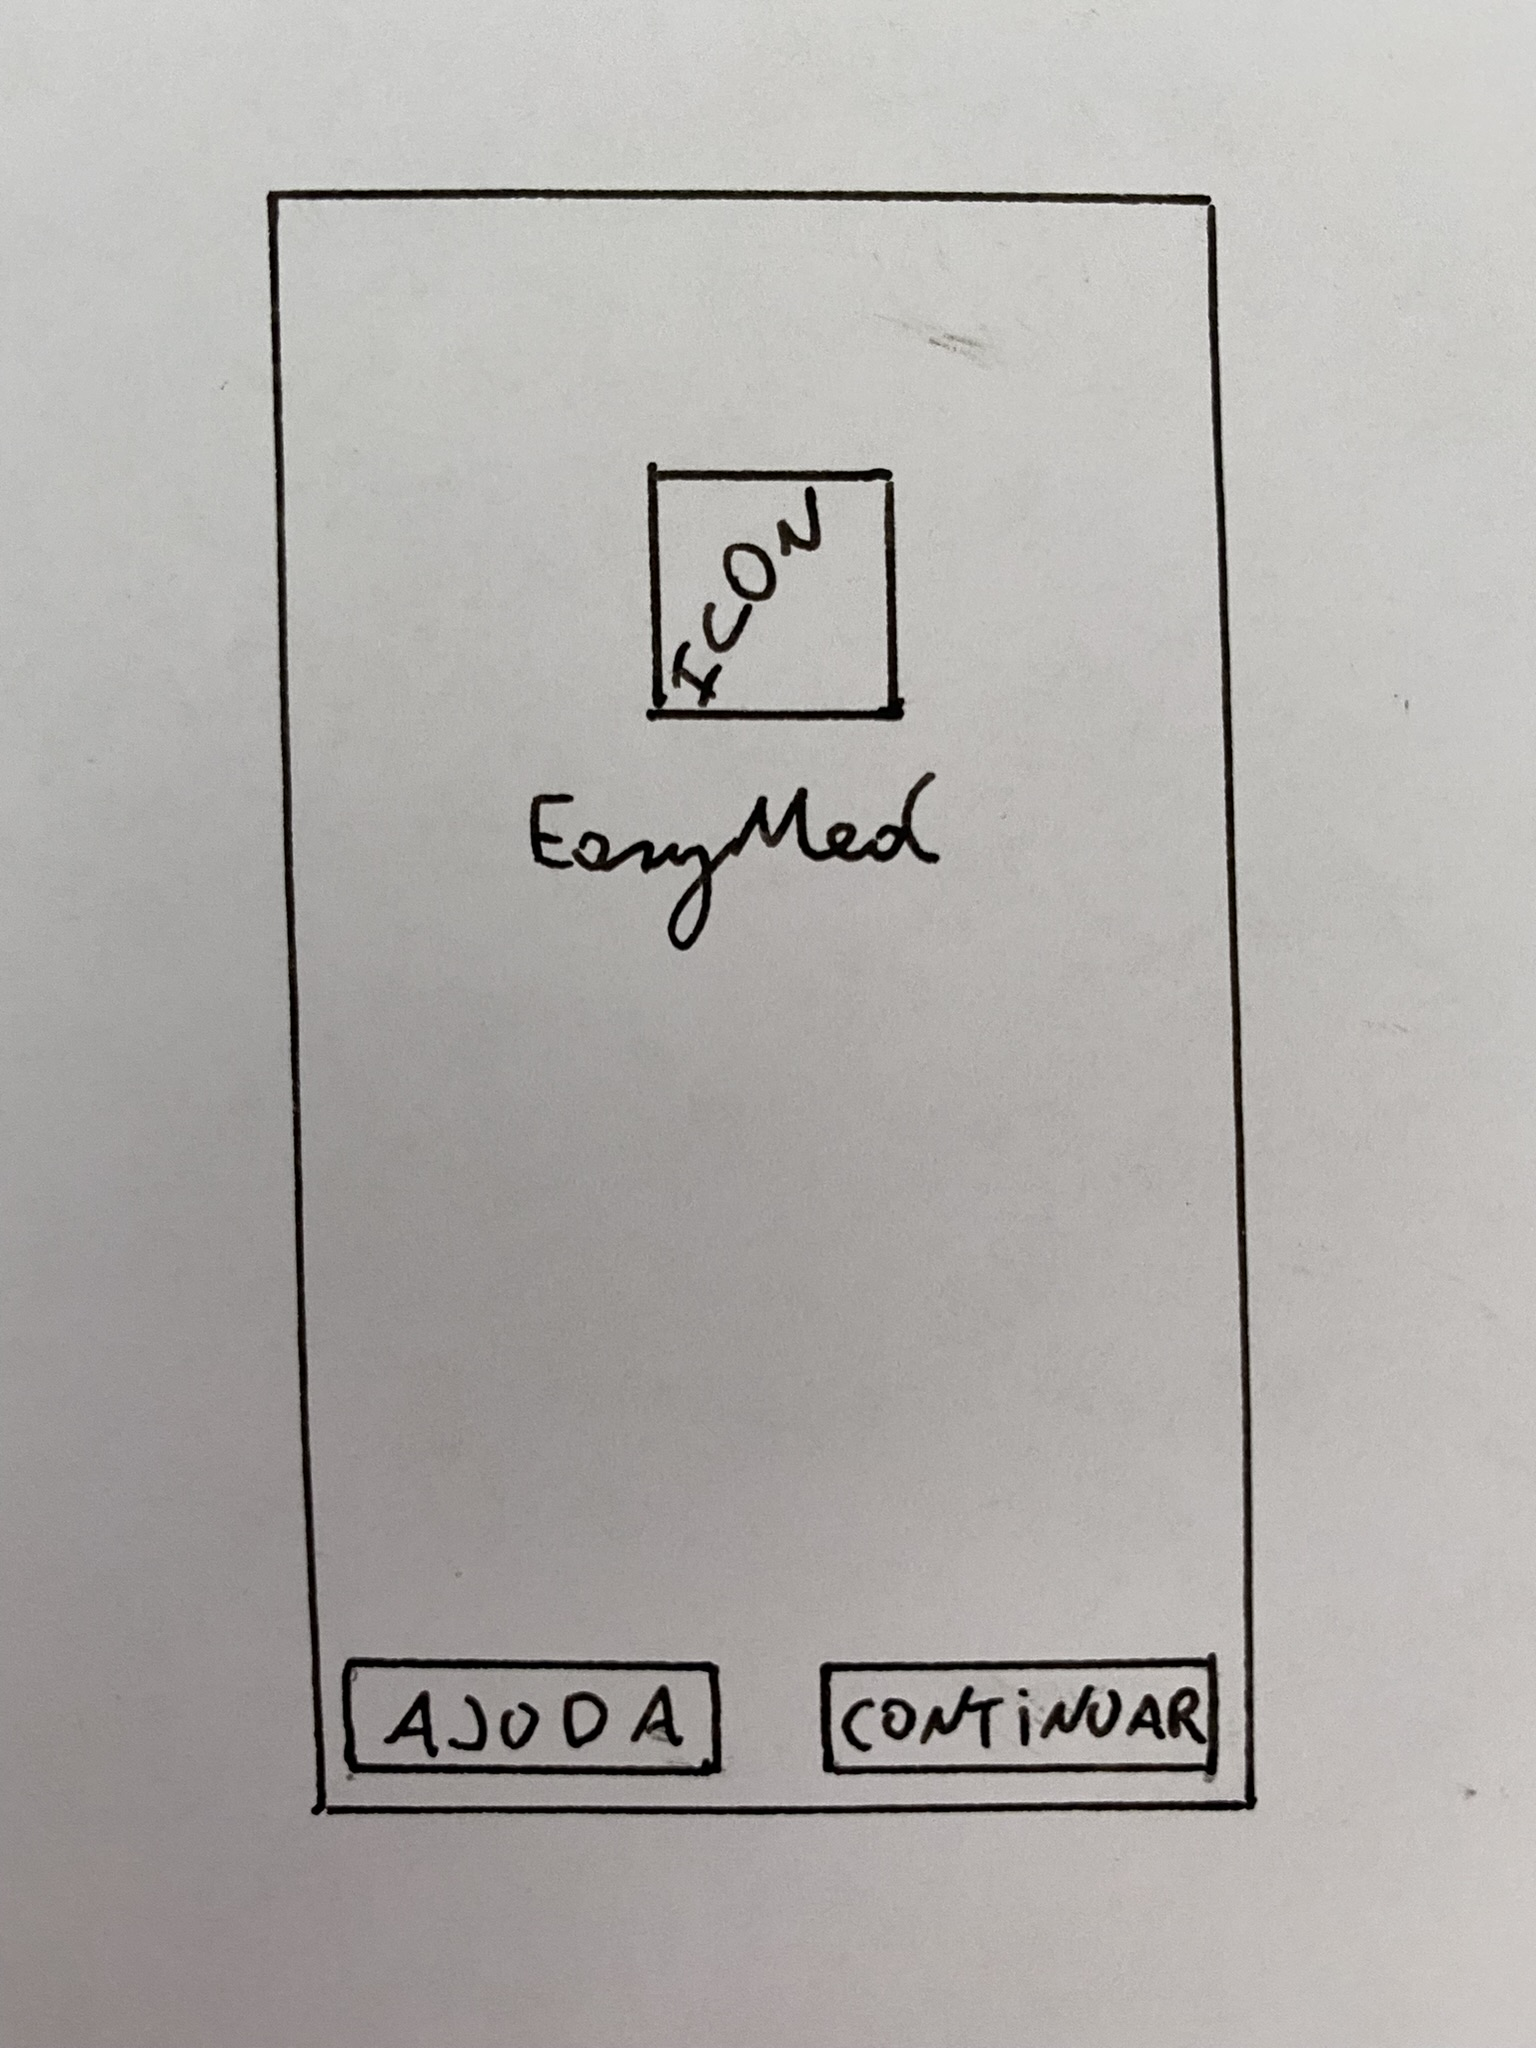
\includegraphics[scale=0.23]{figuras/initialScreen.JPEG}}
    \caption{Ecrã inicial da aplicação, apresentado após a mesma ser instalada.}
    \label{fig:first_screen_inicial_screen}
\end{figure}

\newpage

\begin{figure}[H]
    \centering
    \shadowbox{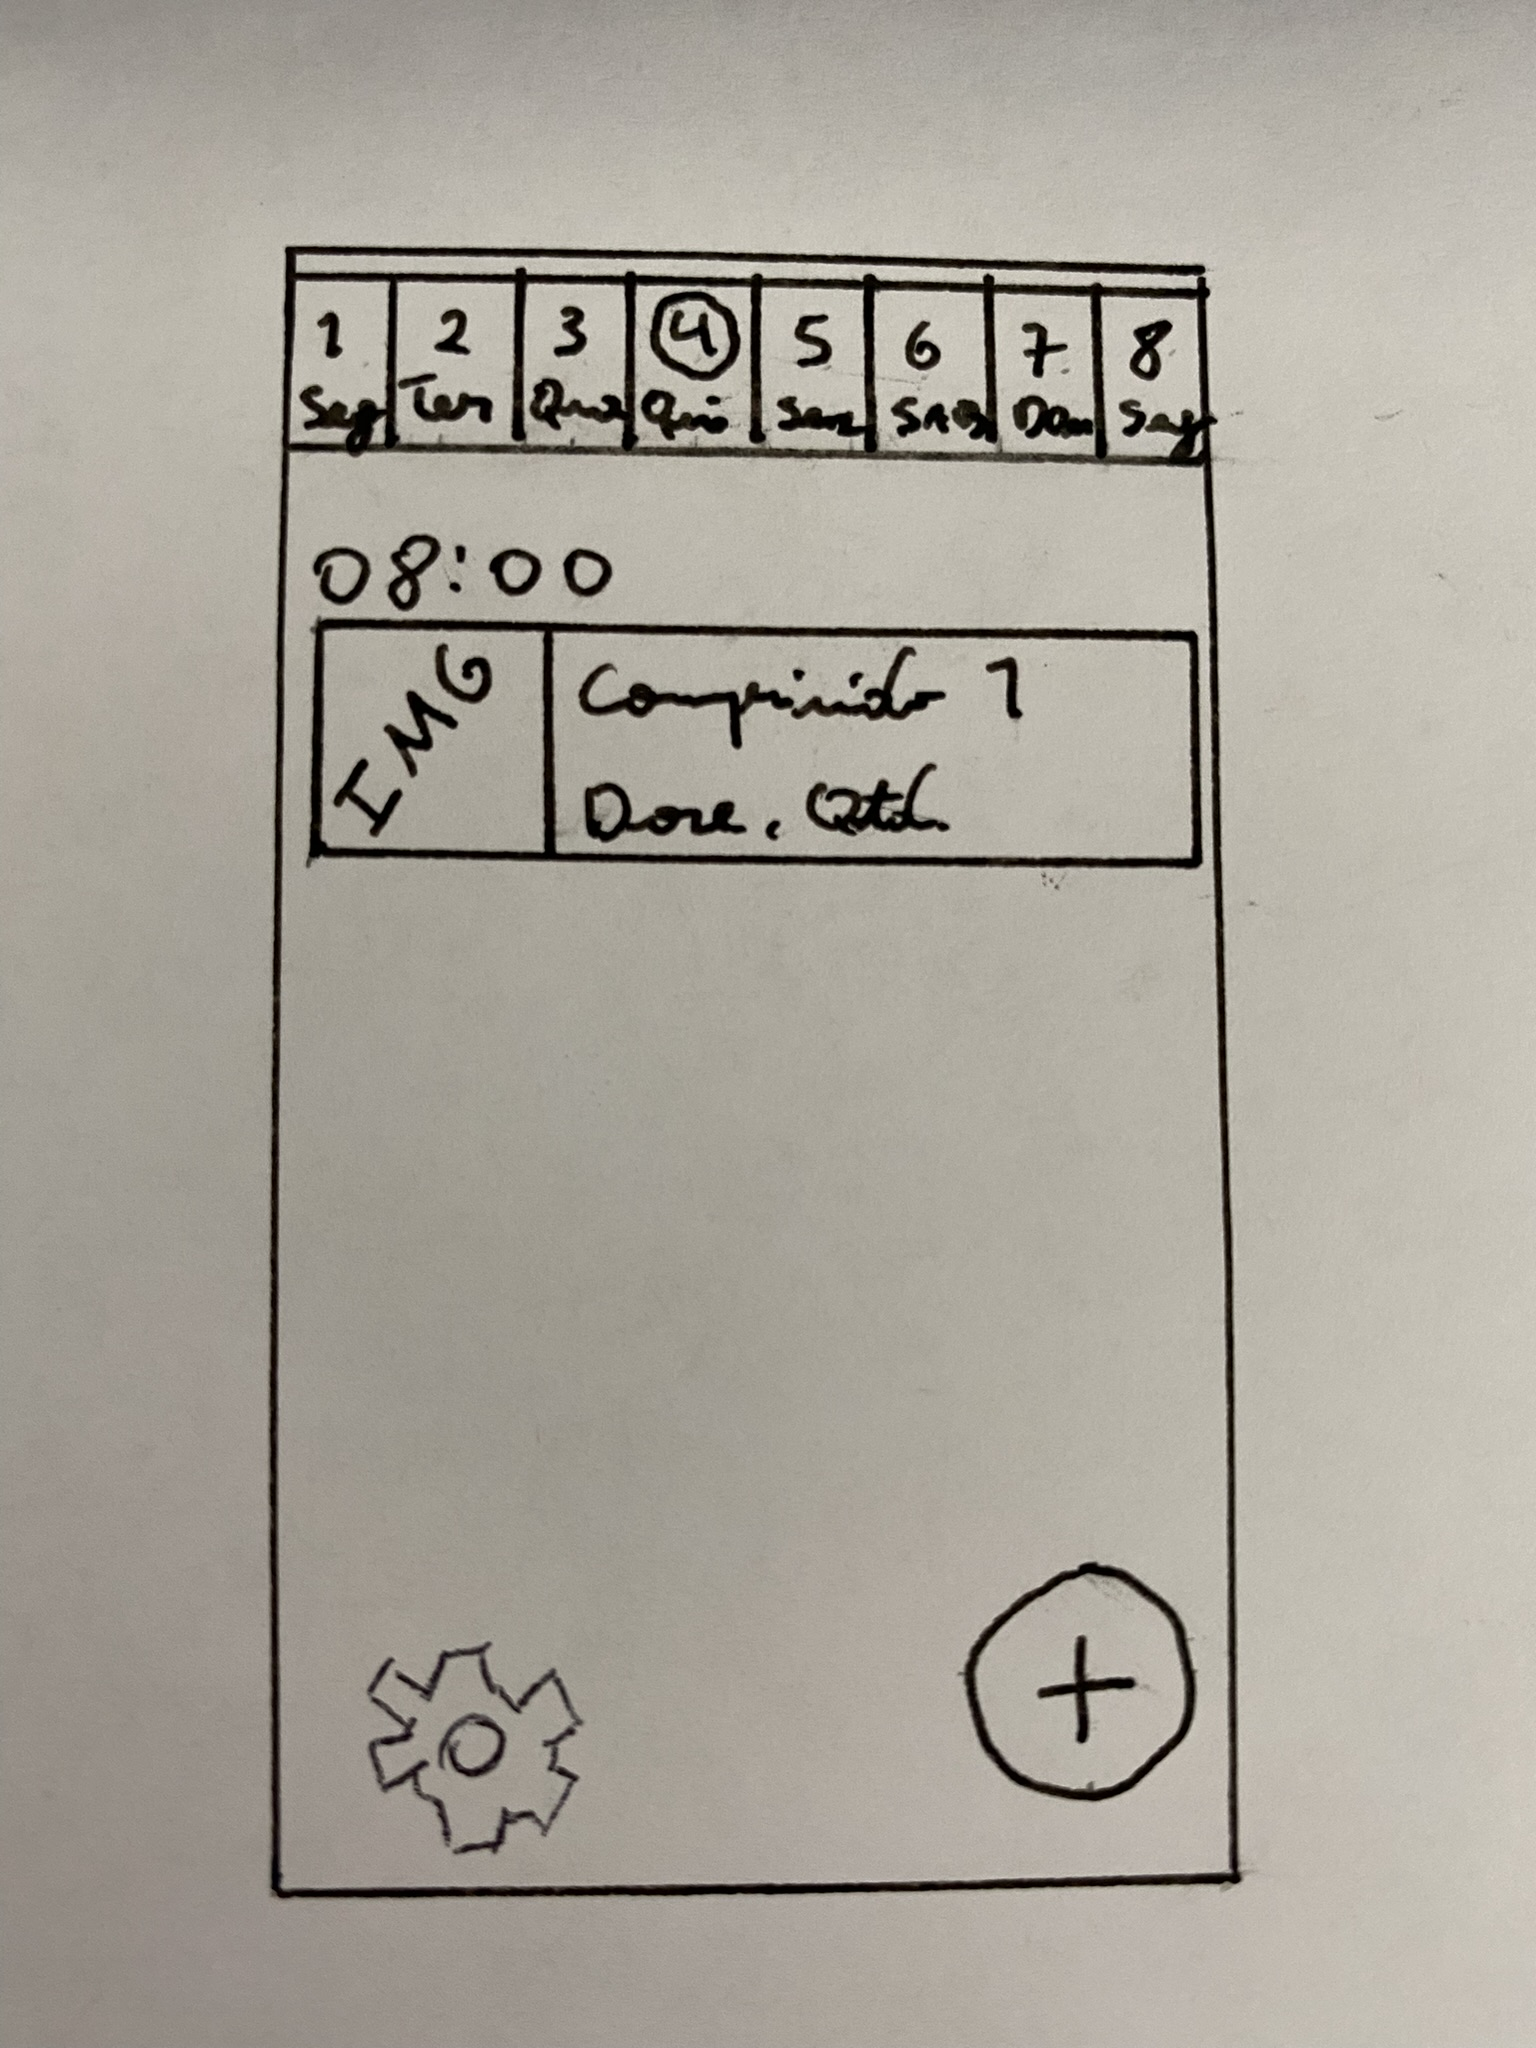
\includegraphics[scale=0.25]{figuras/home2.jpeg}}
    \caption{Ecrã Principal da Aplicação.}
    \label{fig:second_screen_main_screen}
\end{figure}

\newpage

\begin{figure}[H]
    \centering
    \shadowbox{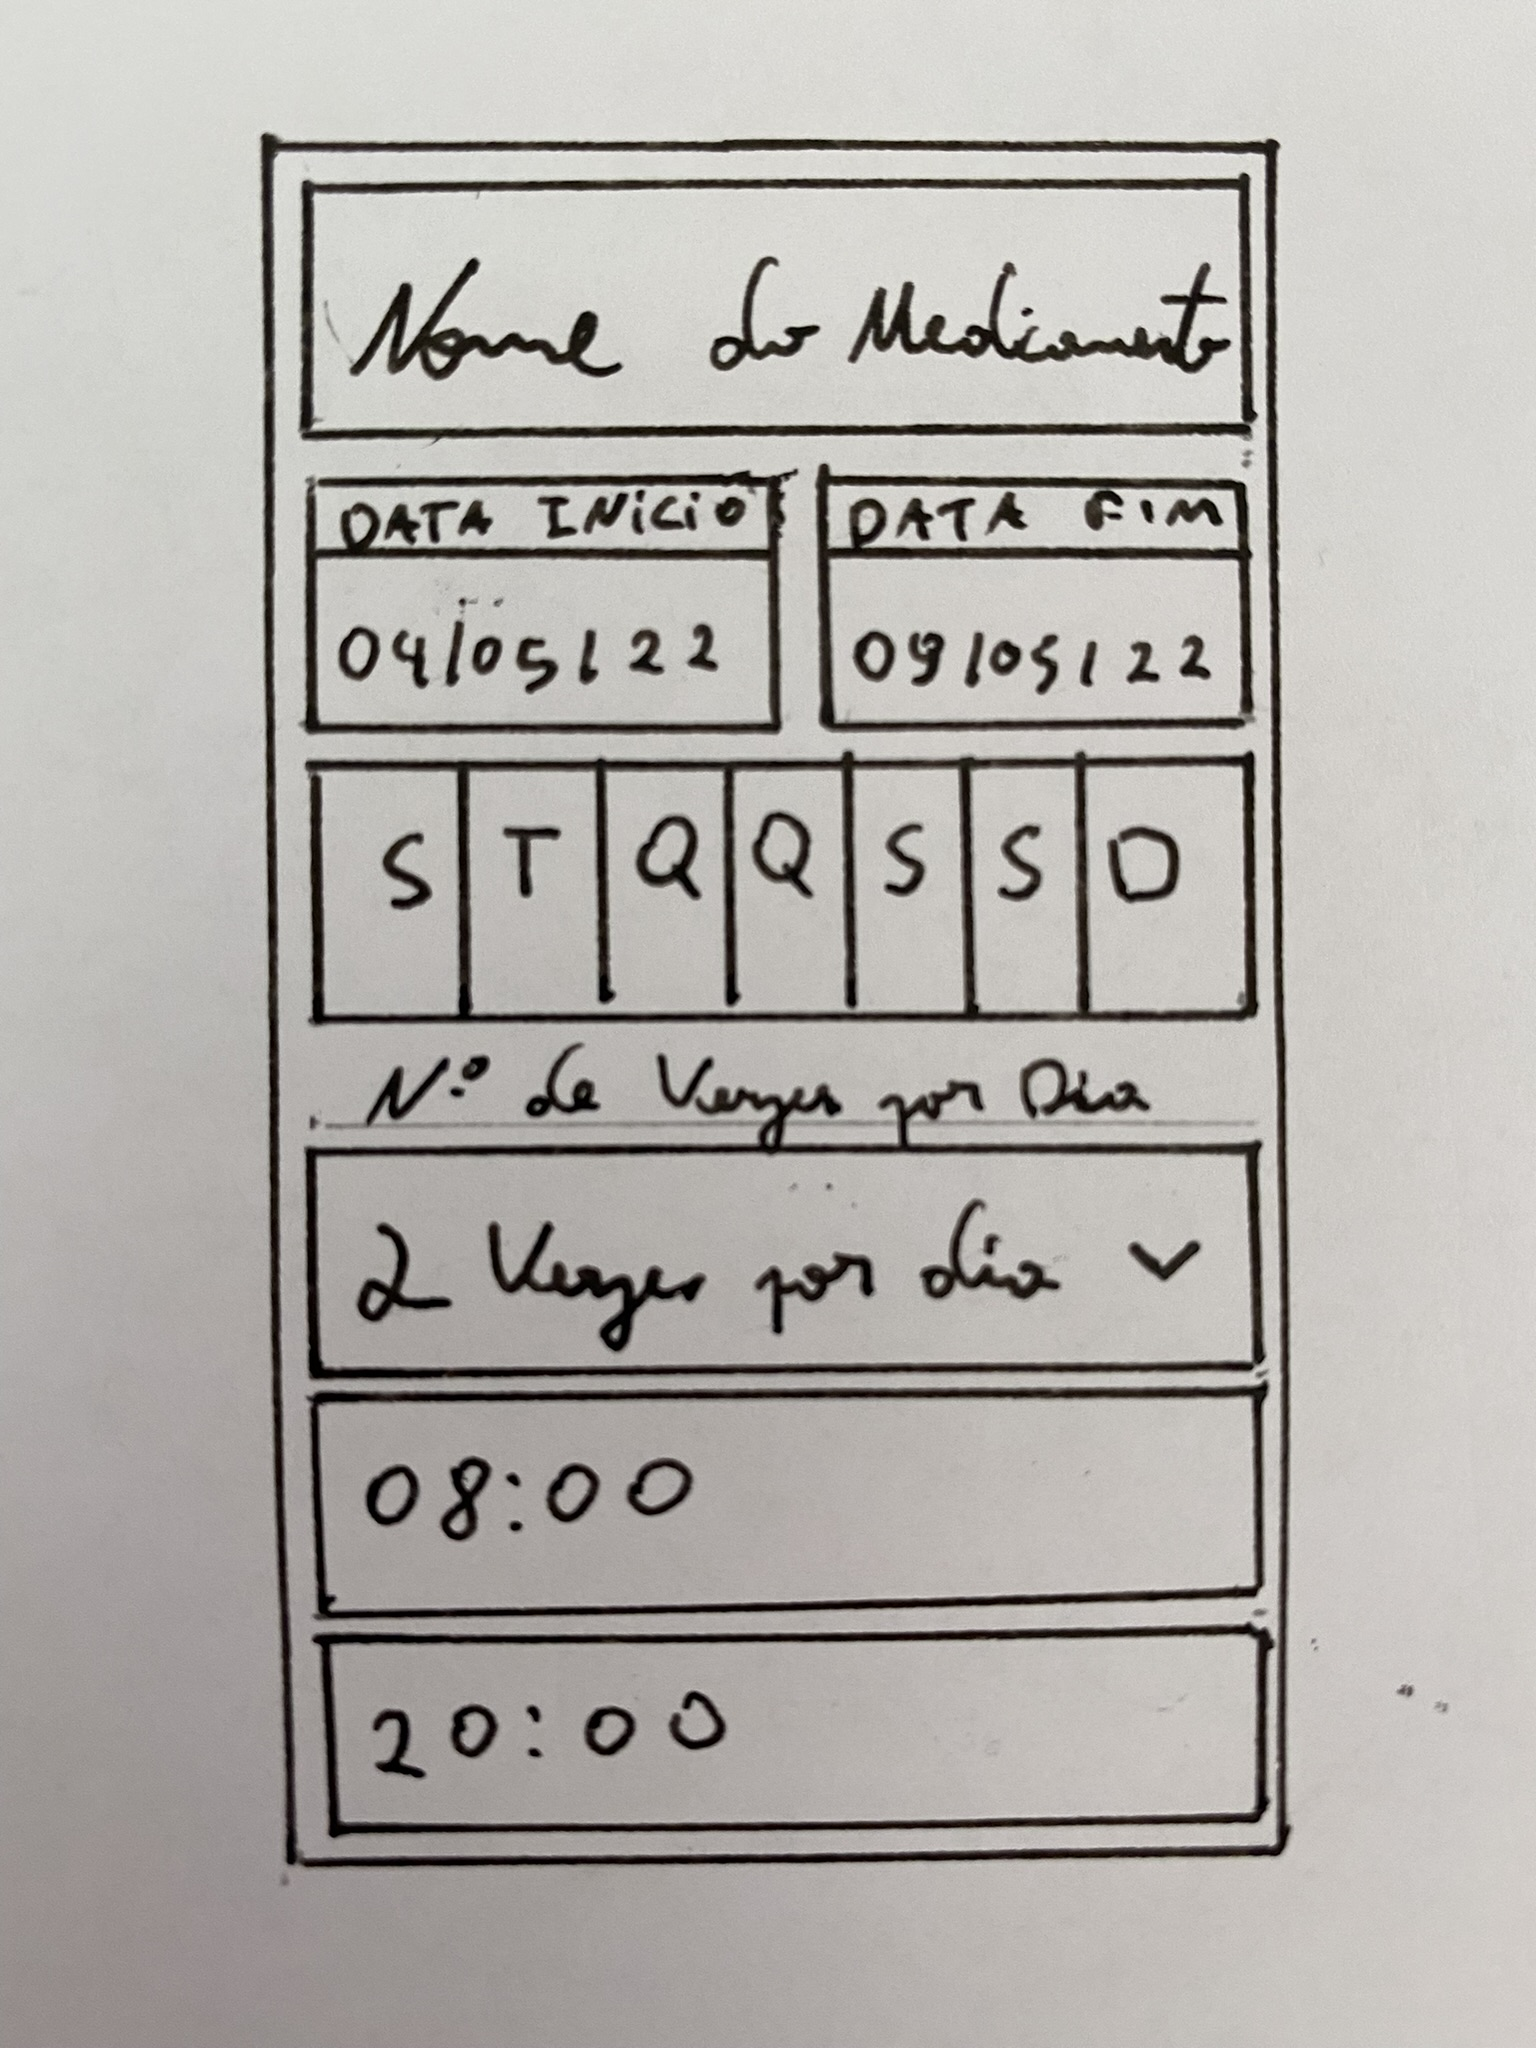
\includegraphics[scale=0.25]{figuras/addRemindeUI.JPEG}}
    \caption{\textit{UI} para Adição de Lembretes.}
    \label{fig:third_screen_add_remainder}
\end{figure}

\newpage

\subsection{Diagramas ilustrativos da navegação na aplicação \textit{EasyMed}}
Nesta secção iremos apresentar os nossos \textit{designs} finais que irão demonstrar como funcionará a navegação dentro da nossa aplicação.

\subsubsection{Primeiro Ecrã}
Neste primeiro ecrã, inicial/"boas vindas" é nos apresentado o ícone do aplicação e dois botões, um de "Ajuda" e um de "Continuar", este primeiro abre uma janela com algumas informações acerca da aplicação, o segundo vai abrir o segundo ecrã principal da aplicação (\ref{fig:second_screen_initial_screen_android_studio})
\begin{figure}[H]
    \centering
    \shadowbox{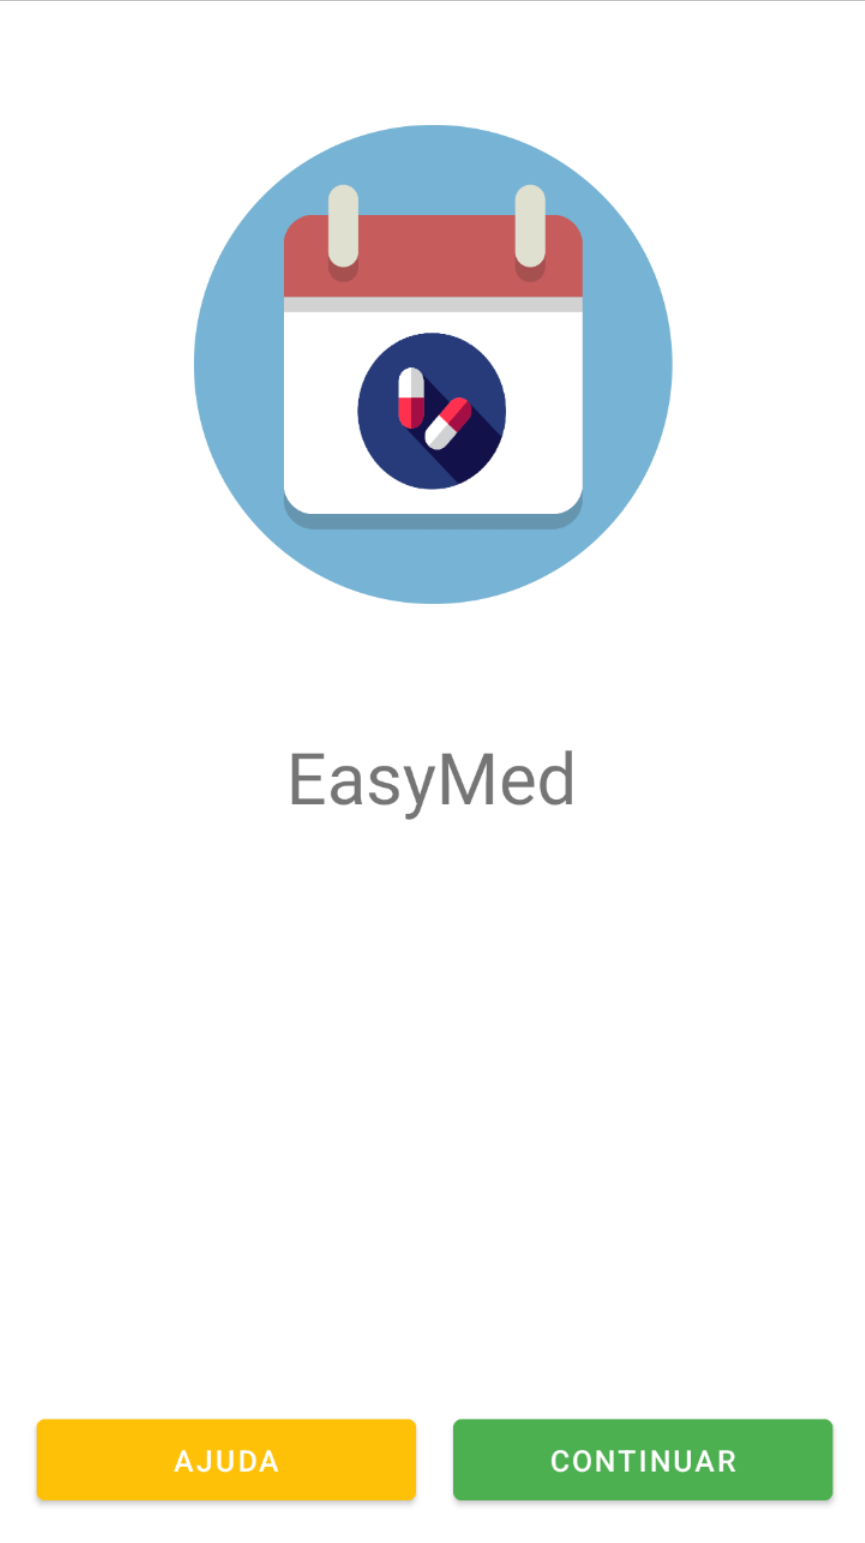
\includegraphics[scale=0.5]{figuras/initialScreenAndroidStudio.png}}
    \caption{Ecrã Inicial da Aplicação}
    \label{fig:fisrt_screen_initial_screen_android_studio}
\end{figure}

\pagebreak

\subsubsection{Segundo Ecrã}
No segundo ecrã temos um \textit{slider} com os dias da semana presente com os dias do mês com o dia selecionado, o atual por \textit{default}, mais a baixo temos o horário da toma dos medicamentos do dia selecionado.\\
O botão do canto inferior esquerdo levo o utilizador para as definições da aplicação, o da direita é destinado a adicionar outros medicamentos e leva para o terceiro ecrã (\ref{fig:third_screen_initial_screen_android_studio}).
Selecionar algum dos medicamentos presentes neste ecrã permite também editar as informações dos mesmo.
\begin{figure}[H]
    \centering
    \shadowbox{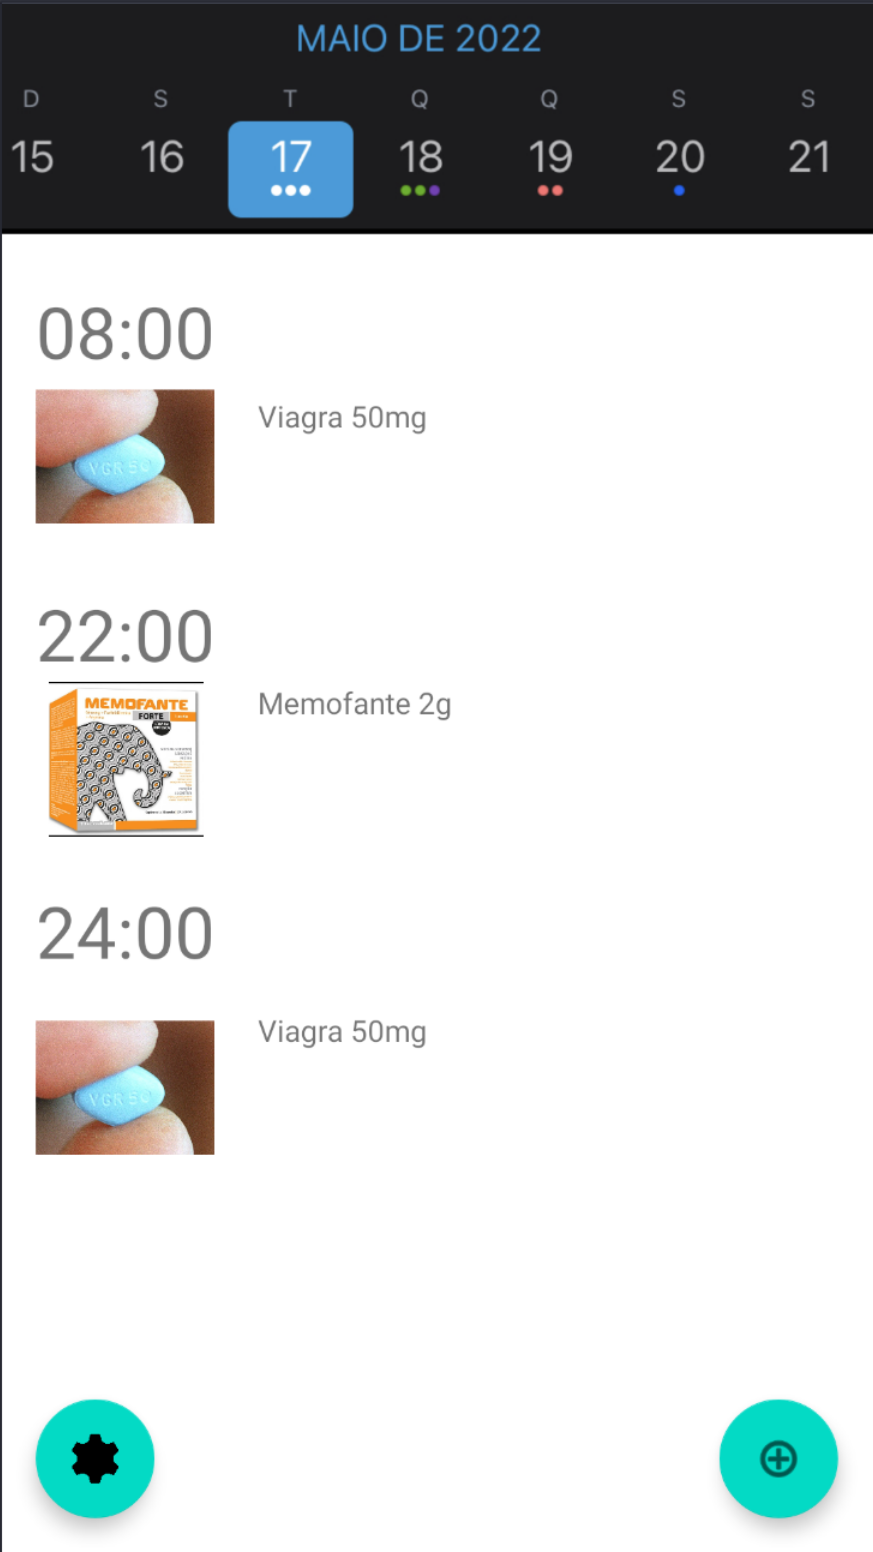
\includegraphics[scale=0.5]{figuras/second_screen_ui.png}}
    \caption{Ecrã Principal da Aplicação}
    \label{fig:second_screen_initial_screen_android_studio}
\end{figure}

\pagebreak

\subsubsection{Terceiro Ecrã}
O terceiro e ultimo ecrã serve para adicionar um medicamento vindo do segundo ecrã introduzindo o nome, data de inicio e fim, os dias para tomar o medicamento e o numero de vezes por dia com os respectivos horários.\\
Depois de introduzir a informação acima referida o utilizador têm dois botões para aplicar a adição desse medicamento ou cancela-la.

\begin{figure}[H]
    \centering
    \shadowbox{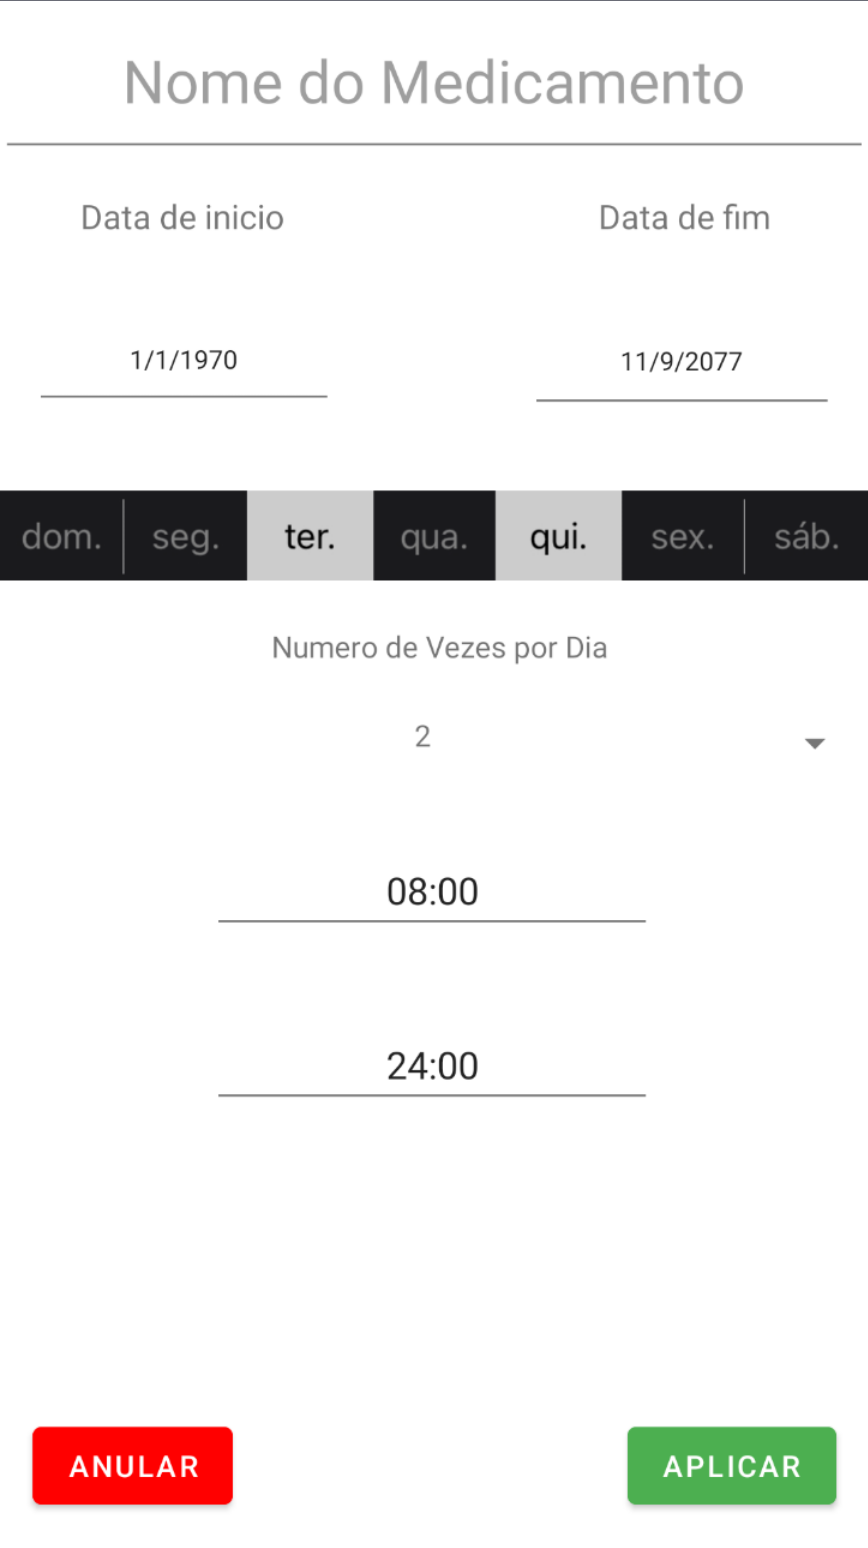
\includegraphics[scale=0.5]{figuras/third_screen.png}}
    \caption{Ecrã de Adição de Lembretes}
    \label{fig:third_screen_initial_screen_android_studio}
\end{figure}

Os esboços anteriores estão no repositório criado para este projeto \cite{easymed}.

\newpage

\section{Regras de usabilidade}\label{section:usability_rules}
\subsection{Iniciativa de diálogo}
Apresenta iniciativa de diálogo no primeiro ecrã (\ref{fig:fisrt_screen_initial_screen_android_studio}) quando nos dá as duas opções de "continuar" para o ecrã seguinte ou selecionar a opção de "ajuda" caso esta seja necessária.

\subsection{Recuperabilidade}
Esta aplicação apresenta o princípio de recuperabilidade no terceiro ecrã (\ref{fig:third_screen_initial_screen_android_studio}) onde apresenta o botão "anular" que permite ao utilizador voltar a introduzir as informações em caso de erro.

\subsection{Personalização}
Esta aplicação apresenta o princípio de personalização porque conseguimos customizar completamente as opções presentes no nosso terceiro ecrã (\ref{fig:third_screen_initial_screen_android_studio}) onde podemos fazer a edição do nome do medicamento, datas, horas e vezes por semana que o medicamento tem que ser tomado.

\subsubsection{Observabilidade}
Esta aplicação apresenta o princípio de observabilidade porque no segundo ecrã (\ref{fig:second_screen_initial_screen_android_studio}) podemos observar todos os medicamentos adicionados pelo utilizador bem como uma fotografia dos mesmos.

\subsubsection{Conformidade de Funcionalidades}
A nossa aplicação possui um leque de funcionalidades bastante diversas que permite aos nossos utilizadores realizarem com facilidade as tarefas previstas. 

\newpage

\section{Conclusão}\label{section:summary}
A realização deste trabalho deu nos a entender que o processo de desenvolvimento de uma aplicação é mais trabalhoso e longo do que tínhamos antecipado antes de o iniciarmos, pois antes sequer de se iniciar a fazer o \textit{design} e escolher as funcionalidades temos que fazer uma caracterização de para quem queremos desenvolver a aplicação, e que funcionalidades essas mesmas gostariam ver implementadas.\\
Apenas após estes passos iniciais é que podemos seguir para a fase de \textit{design} dos ecrãs, que foi a fase final deste trabalho em especifico, numa fase seguinte iriamos começar a fazer a implementação desses designs no \textit{Android Studio\texttrademark}, e dó código que os fará funcionar, seguido depois de uma fase de testes com os utilizadores alvo antes de ser lançada para o mercado.\\
Podemos concluir que com este trabalho aprofundamos muito o nosso conhecimento sobre este tema e cada uma das suas diferentes fases de desenvolvimento.

\newpage


\bibliographystyle{plain}
\bibliography{references}

\end{document}
